\section{Building pangenomic models}

\subsection{Constructing graphs} 
% Robin


\subsection{Indexing genome graphs}

A text index maps query strings to their occurrences in the indexed text. The occurrences are typically reported as a list of starting positions, from which one can easily determine the substrings matching the query.

Indexing the sequences encoded in a graph is more involved. The number of $k$~bp paths often grows exponentially in $k$, and the number of distinct $k$-mers encoded as path labels may also grow exponentially. Indexing or even enumerating all $k$-mers in the graph may be infeasible for reasonable values of $k$. And if the starting position of the occurrence reported by the index is in a complex region of the graph, there may be an exponential number of $k$~bp paths to investigate.

In practice, indexes for genome graphs must make trade-offs not encountered in text indexes. In order to limit the exponential growth, the index may only support relatively short query strings. Some indexes support longer queries by doing extensive preprocessing. In other indexes, queries mapping to complex graph regions can be slow. Instead of indexing the entire graph, the index may only contain $k$-mers from a simplified graph, or from specific paths of the graph. And while finding the path matching the query may be expensive in some cases, indexes typically save space by only reporting the starting position of the match.

\subsubsection{Indexing sequences using a graph}

The FM-index \cite{Ferragina_2005} is a text index based on the Burrows--Wheeler transform (BWT) \cite{Burrows_1994} that is frequently used with DNA sequences. A variant of the FM-index, the RLCSA \cite{Maekinen_2010}, run-length encodes the BWT, allowing it to store and index a collection of similar sequences space-efficiently. Huang et~al.\ \cite{Huang_2010} observed that if we know a good global alignment of the sequences, we can use that information to make the index both smaller and faster. Na et~al.\ \cite{Na_2016,Na_2018} developed this approach further in their FM-index of alignment. While the articles do not mention it, both Huang et~al.\ and Na et~al.\ use the graph induced by the alignment as a space-efficient representation of the sequences.

\subsubsection{Acyclic graphs}

% TODO "VCF graph" is a placeholder
GenomeMapper \cite{Schneeberger_2009} was the first graph-based read aligner. It builds a directed acyclic graph from a reference sequence and a set of variants (VCF graph). To index the graph, GenomeMapper uses a simple hash-based $k$-mer index, with $k \le 13$ to limit memory usage.

GCSA \cite{Siren_2014} was the first attempt to use the BWT with graphs. It takes either a prebuilt DAG or generated one from a multiple alignment of sequences. GCSA then applies a number of graph transformations that preserve the path labels in the graph, until the nodes can be unambiguously sorted by the labels of the paths starting from the node. This process balances on the fine line between linear and exponential. If the complexity of the graph is above a critical threshold, the transformed graph quickly becomes too large to handle.

BWBBLE \cite{Huang_2013} is a BWT-based representation for VCF graphs. Simple substitutions are encoded in the sequence using IUPAC codes, and the sequence is indexed using a normal FM-index. Because each base can be encoded using 8 different characters, the search branches after every base. Most branches can be quickly eliminated, however. Insertions and deletions produce separate sequences, with selected amount of context around the variant. The length of this context is an effective upper bound for query length.

The vBWT \cite{Maciuca_2016} took another approach to using the BWT for indexing VCF graphs. It encodes variants as \texttt{(ref|alt1|\dots)} in the sequence. When the search encounters a variant, it must branch to handle each allele separately. While both BWBBLE and vBWT trade faster index construction for slower queries, a combination of the ideas can be quite practical \cite{Buechler_2019}.

\subsubsection{General graphs}

Some text indexes are based on Lempel--Ziv parsing or context-free grammars. These indexes first find partial matches between the query string and the indexed phrases and then combine the partial matches into full matches using two-dimensional range queries. In the hypertext index \cite{Thachuk_2013}, each node is a separate phrase. Queries mapping to a single node or crossing a single edge can be matched efficiently, while finding mappings to complex graph regions can be slow.

Bowe et~al.\ \cite{Bowe_2012} used techniques similar to GCSA for representing de Bruijn graphs. If the graph transformations used in GCSA construction are stopped after $i$ steps, the resulting graph is equivalent to an order-$2^{i}$ de~Bruijn graph. This de~Bruijn graph can be used to approximate the original graph. There are no false negatives, but matches longer than $2^{i}$ may be false positives. By using this approach, GCSA2 \cite{Siren_2017} attempts to support fast queries in arbitrary graphs.

While stopping the construction early allows GCSA2 to handle more complex graphs than GCSA, most graphs must be simplified before they can be indexed. Typical simplifications include removing high-degree nodes and complex regions from the graph and replacing them with the reference sequence. If a collection of haplotypes is available, the removed regions can be replaced with new subgraphs that contain separate paths for each distinct local haplotype \cite{Siren_2019}. This way, the index will contain all $k$-mers from the haplotypes, while usually missing $k$-mers from their recombinations.

\subsubsection{Indexing graphs using sequences}

Instead of attempting to index the entire graph, it is often sufficient to index only selected paths in it. CHOP \cite{Mokveld_2018} takes the paths corresponding to haplotypes and breaks them into smaller pieces. The distinct pieces form an artificial linear reference, which can be used with any read aligner. The process guarantees that any substring of the haplotypes of length $k$ is also a substring of one of the pieces. As with BWBBLE, $k$ represents an effective upper bound for query length.

The Pan-genome Seed Index (PSI) \cite{Ghaffaari_2019} follows a similar approach with artificial paths. Instead of using haplotypes, PSI uses a greedy algorithm to find a set of paths that covers as many $k$~bp windows in the graph as possible. An index using these paths alone already works well in practice.

When a fully sensitive index is needed, PSI can reverse the role of the query strings and the graph. While complex graph regions may contain an excessive number of $k$-mers, the reads mapping to them only contain a limited number of $k$-mers. By indexing a batch of reads and searching for the complex regions in that index, all mappings of the query strings to the graph can be found with reasonable resources.


\subsection{Other population-ish succinct data structures}
% Erik / Jouni?

\subsubsection{de Bruijn}

% BOSS: \cite{Bowe_2012} (\cite{Roedland_2013} is similar)

\subsubsection{VCFs / genotype calls / haplotypes / binary matrices}

\subsubsection{gPBWT, GBWT}

% Jouni: I can write this

\subsubsection{Alignments / collections of strings}

% Jouni: We probably don't have space for this.


\section{Finding structure in the model}

\subsection{Visualization}
% Adam

Once one has constructed a graph pangenomic model, one might want to look at it.
A number of tools have been developed for this purpose.

Bandage (\textbf{B}ioinformatics \textbf{A}pplication for \textbf{N}avigating \textit{\textbf{D}e novo} \textbf{A}ssembly \textbf{G}raphs \textbf{E}asily) \citep{Wick_2015} is one of the most popular \citep{Mikheenko_2019}.
Originally designed for working with bacterial assembly and meta-assembly graphs \citep{Wick_2015}, it supports a wide range of formats and graph  paradigms.
It can be effectively used for interactively visualizing and exploring subregions of human-scale pangenome graphs \citep{Garrison_2019}, but its shortcomings become apparent at larger scales or with higher degrees of connectivity between graph regions \citep{Mikheenko_2019}.
The tool does have support for restricting the portion of the graph displayed to a particular ``scope'', but the tool is fundamentally built around laying out the graph under study in two dimensions, with all nodes represented, and panning and zooming around it.
Moreover, while the tool includes the ability to search for sequences in the graph, it does not have any ability to structure graph display using known linearization information.
Additionally, Bandage is implemented as a cross-platform native C++/Qt application \citep{Wick_2015}, which allows the tool to be self-contained but precludes the use of cloud resources for dealing with larger graphs; all graph data must be stored and processed on the user's machine at visualization time.

GfaViz is another C++/Qt application for visualizing genome graphs which claims full support for newer GFA2 features, such as the gaps which allow GFA2 to represent scaffold graphs in addition to assembly graphs; these features are not available in Bandage, which supports only GFA1 \citep{Gonnella_2018}.
However, unlike Bandage, the GfaViz project has not released any binary builds or user interface screenshots of their application, so Bandage remains the more accessible tool.

Departing from the desktop application model, two recent graph visualization tools, \textbf{S}caffold \textbf{G}raph \textbf{T}ool\textbf{K}it (SGTK) and \textbf{A}ssembly \textbf{G}raph \textbf{B}rowser (AGB), adopt a build-a-web-page model, in which a web-based visualization is prepared that does not rely on further server support, lowering end-user system requirements \citep{Kunyavskaya_2018,Mikheenko_2019}.
SGTK is designed for visualizing scaffold graphs, which can have negative-overlap gaps between sequenced segments, and is based around the in-browser Cytoscape.js graph layout and rendering library \citep{Kunyavskaya_2018}.
It includes a potentially highly interpretable, reference-sequence-structured ``browser'' layout, but its use of Cytoscape.js appears to push it towards a generic circular node representation, rather than the noodles of Bandage \citep{Kunyavskaya_2018}.
Moreover, its authors do not demonstrate its usability on large graphs, with the largest graph evaluated having only 923 nodes and 60,679 edges \citep{Kunyavskaya_2018}.

AGB has a similar overall design to SGTK, but makes different implementation choices.
It is relatively tightly tied to the assembly graph use case, requiring each (sequence-bearing) edge to be classifiable as ``unique'' or ``repetitive'' based on assembler annotation or sequencing coverage \citep{Mikheenko_2019}.
Where SGTK used Cytoscape.js, AGB relies on the venerable \texttt{graphviz} tool itself, compiled for execution in the browser \citep{Mikheenko_2019, Ellson_2001}.
This lets it lay out graphs in a more flow-guided way, using graphviz's rank-based algorithms, as compared to Cytoscape.js's more force-directed-looking layouts \citep{Mikheenko_2019, Kunyavskaya_2018}.
AGB is built around the idea of splitting up an assembly graph and visualizing portions of it, and features many ways to do this, including linear-reference-based and minimum-edge-cut-based approaches \citep{Mikheenko_2019}.
On the backend, the tool is built around potentially megabyte-scale JSON files \footnote{\url{https://github.com/almiheenko/almiheenko.github.io/blob/8f4b2f8c7c498f04fa32f53f69b4bc59888a14f0/AGB/Flye_Human/data/repeat_graph.json}}, with no apparent provision for region-specific download, but the tool is still demonstrated to be scalable enough to handle human and other eukaryotic assembly graphs \citep{Mikheenko_2019}.

There is a difference in scale when moving from an assembly or scaffold graph to a comprehensive pangenome graph for even a species with as little diversity as humans.
While tools like SGTK and AGB have been demonstrated on graphs with tens of thousands of entities, the 1000 Genomes Project dataset contains 88 million known human variants \citep{1000_2015}, which gives a density over the 3 billion base human genome of about 34 bases per variant, and a comprehensive pangenome graph with tens to hundreds of millions of elements---a much larger graph than those that SGTK and AGB have been shown to work with.
Moreover, to achieve their single-megabyte-scale visualization file sizes for hundred-megabase- to gigabase-scale assemblies, these tools necessarily elide sequence information.

To deal with comprehensive pangenome graphs with sequence data, one design approach is to keep the browser-based client but to put more intelligence into the server.
This is the avenue taken by the Sequence Tube Map, which renders regions of pangenome graphs using a visual language inspired by transit system maps \citep{Beyer_2019}.
This tool operates at a much more magnified zoom level than tools designed to work with assembly graphs, and is useful for visualizing base-scale variation and short read mapping locations in human-chromosome-scale graphs \citep{Beyer_2019}.
However, its imposition of a local linear ordering and its limited graph simplification tools make it difficult to use on larger regions \citep{Beyer_2019}.
Additionally, its architectural decision to load the graph from disk for every request makes latency prohibitively high when working with combiend graphs above the scale of a single chromosome, so the tool is not suitable for graphs which cannot be broken up into chromosome-scale connected components.

Other approaches to visualizing comprehensive pangenome graphs rely on restricting the problem in order to improve efficiency.
For example, by forcing the sequence-bearing nodes of the graph into a one-dimensional layout, and producing vector rather than raster output, the \texttt{vg viz} tool promises to render graphs of arbitrary size and complexity in linear time \citep{Garrison_2019}. The intended use case seems to be to use a single global linearization, and to interactively render regions of it for display, but it is also possible to non-interactively render an entire graph to a very large image \citep{Garrison_2019}. The tool is designed around a base-level visual representation of the graph, and optimized for comparing long embedded paths in the graph, on the basis of which nodes they do or do not visit \citep{Garrison_2019}. However, as with the Sequence Tube Map, it can be difficult to understand high-level or nonlinear structures in such a linearized layout \citep{Garrison_2019}. In contrast to the Sequence Tube Map no provision is made for visualizing short read alignments \citep{Garrison_2019}.

Figure~\ref{fig:visualization} provides a visual overview of the visualization methods surveyed here. It remains an open problem to interactively visualize a comprehensive human pangenome graph, potentially including interchromosomal connections, at a variety of zoom levels, with modestly provisioned end-user hardware.

\begin{figure}[h]
    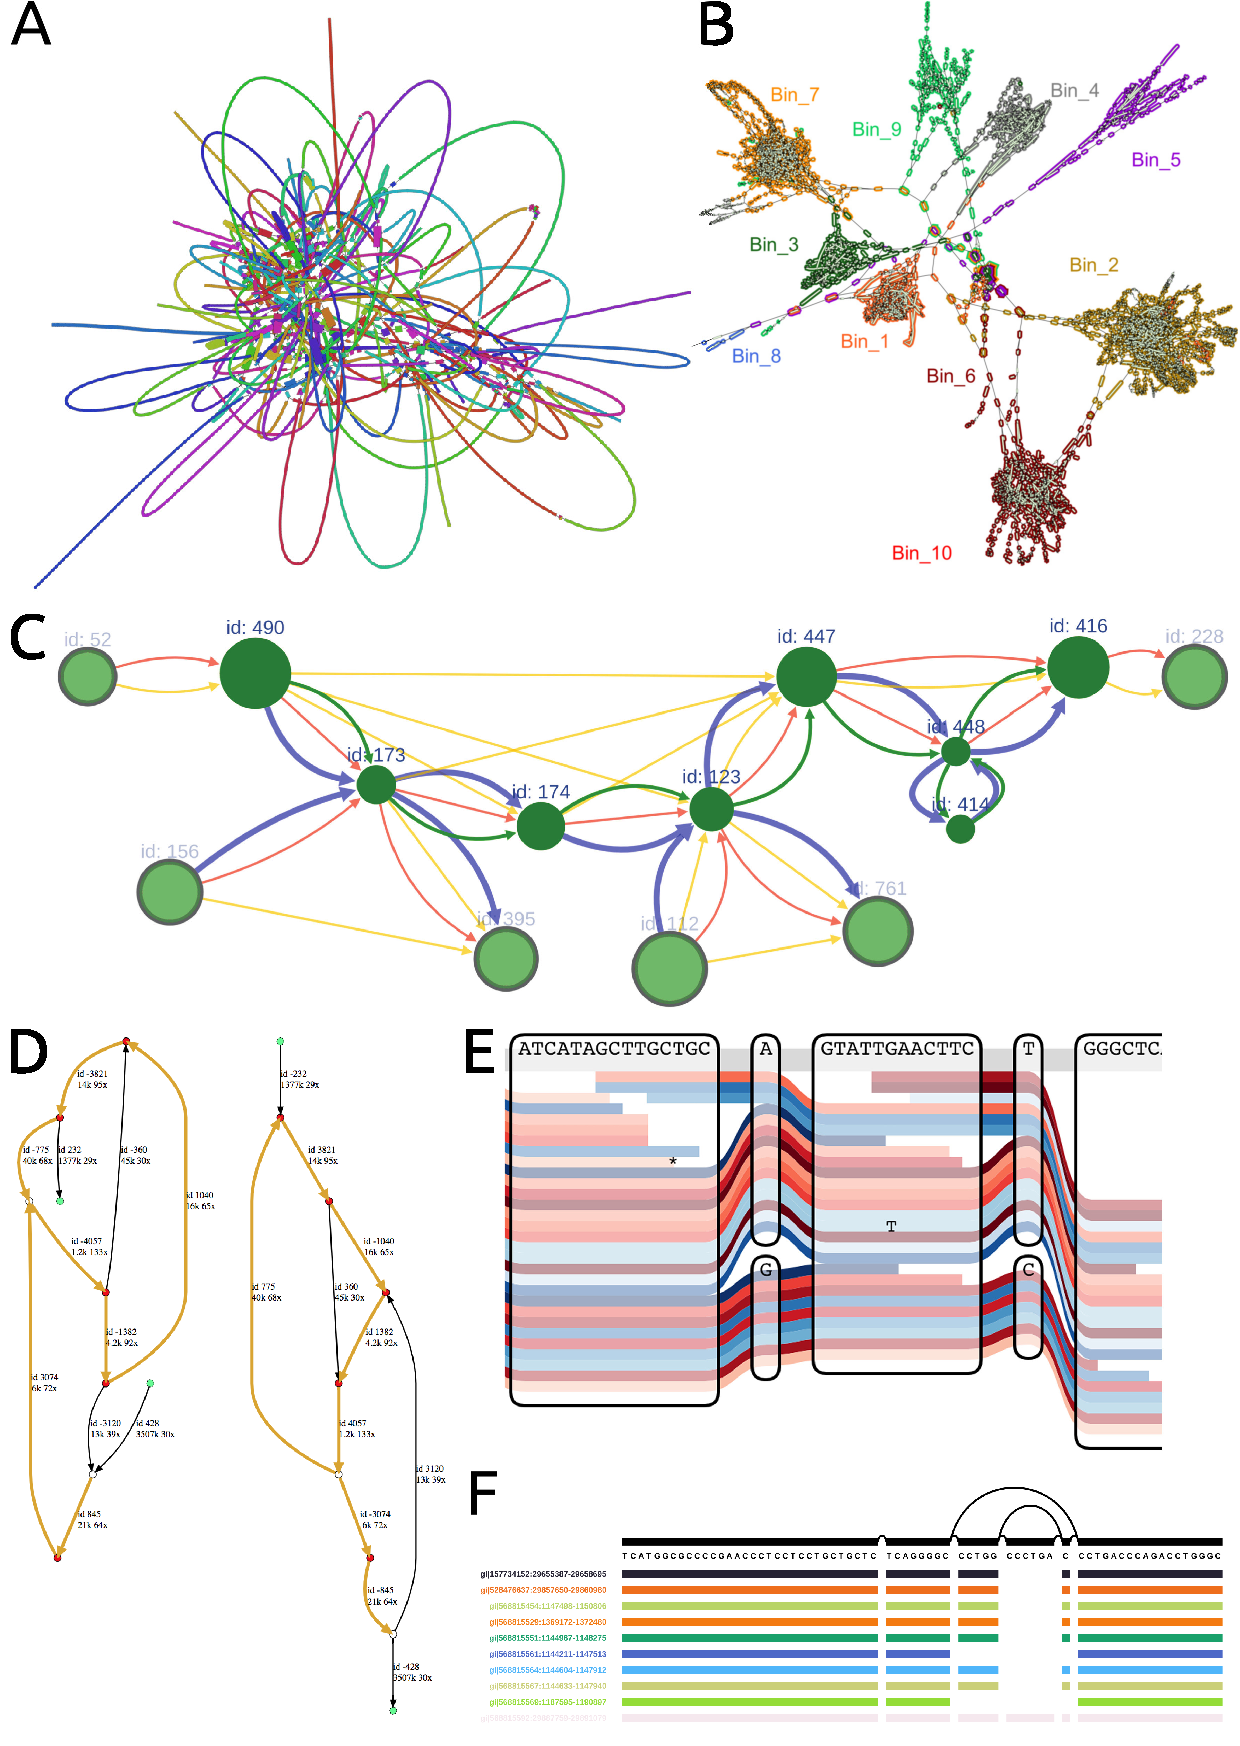
\includegraphics[width=0.9\textwidth]{figures/visualization.eps}
    \caption{\label{fig:visualization} An overview of several approaches to visualizing assembly, scaffold, and comprehensive pangenome graphs. \textbf{A:} Bandage, adapted from \cite{Wick_2015} supplementary section~6. \textbf{B:} GfaViz, adapted from \cite{Gonnella_2018} supplementary figure~S4. \textbf{C:} SGTK, adapted from \cite{Kunyavskaya_2018} figure~1. \textbf{D:} AGB, adapted from \cite{Mikheenko_2019} figure~S3. \textbf{E:} Sequence Tube Map, adapted from \cite{Beyer_2019} figure~2. \textbf{F:} \texttt{vg viz}, adapted from \cite{Garrison_2019} figure~2.20.}
\end{figure}

% Go back and talk about ABySS-Explorer (2009) and its "polar" graphs and wiggly sequence edges?
% Bandage: cross-platform native application
    % Versatile and popular
    % Client-only
    % Could look up a reference but not view vs it
% GfaViz: C++/Qt tool with full GFA1/2 support
    % Has a GUI but no screenshots or binaries
    % Can show cool stuff like reads connected to their assembly contigs
% SGTK
    % build-view model
    % Cytoscape.js or genome browser linear-structured
    % designed for scaffold graphs (more processed?)
    % Not proven on large graphs; only shown going up to 100s of nodes
% AGB: auto-subgraphs (to 100 nodes) and simplifies assembly graphs
    % js GraphViz based
    % Still uses a build-web-page model
    % Kind of tied to assemblies (notion of repetitive vs non-repetitive edges)
    % Can view vs a reference
    % Scales to C elegans at least
        % O(300 * 100 = 30000) nodes
    % Appears to be structured around megabyte-scale GraphViz graphs https://github.com/almiheenko/almiheenko.github.io/tree/master/AGB
        % No LOD-ing on the backend for efficient download, but not a problem at the scale of 10s of thousands.
% Tube Map
    % Client-server model: requires a server, but can use server resources to crunch the graph
    % Designed to impose a left to right local ordering that orients the edges in a hopefully sensible way
    % Scales well to millions of nodes, demonstrated on partial human pangenome graph references


%\citep{Wick_2015} : Bandage
%\citep{Gonnella_2018} : GfaViz
%\citep{Kunyavskaya_2018} : SGTK
%\citep{Mikheenko_2019} : AGB
%\citep{Beyer_2019} : TubeMap
%\citep{Garrison_2019} : Thesis

\subsection{Finding structures in pan-genome graphs}
% Jordan

